%----------------------------------------------------
% Setup Beamer
%----------------------------------------------------
\documentclass[hyperref={colorlinks=true}]{beamer}

%----------------------------------------------------
% Packages to use
%----------------------------------------------------
\input{../packages.sty}

%----------------------------------------------------
% Setup Theme
%----------------------------------------------------
\input{../theme.sty}

%----------------------------------------------------
% Table of Contents at each section transition
%----------------------------------------------------

\AtBeginSection[]
{
   \begin{frame}
       \frametitle{Outline}
       \setcounter{tocdepth}{2}
       \tableofcontents[currentsection]
   \end{frame}
}

%----------------------------------------------------
% Colors
%----------------------------------------------------
\input{../mycolors.sty}

%----------------------------------------------------
% Style, formatting, and new commands
%----------------------------------------------------
\input{../../global.sty}
\input{../newcommands.sty}
\input{../EandMcommands.sty}

%----------------------------------------------------
% Set paths for plots and images
%----------------------------------------------------
\input{../paths.sty}


%-----------------------------------------------------------------------------------------
% Title: [Column]{Title}
%-----------------------------------------------------------------------------------------
\title[PHYS 250 (Autumn 2019) -- Lecture 7]{Ising model (cont'd)}

%-----------------------------------------------------------------------------------------
% SubTitle: [Column]{Subtitle}
%-----------------------------------------------------------------------------------------
\subtitle{PHYS 250 (Autumn 2019) -- Lecture 7}

%-----------------------------------------------------------------------------------------
% Author: [SubAuthor]{Author}
%-----------------------------------------------------------------------------------------
\author[D.W.~Miller]{David Miller}

%----------------------------------------------------
% Institute: [SubInst]{Institute}
%----------------------------------------------------
\institute[EFI, Chicago] 
{
  Department of Physics and the Enrico Fermi Institute\\
  University of Chicago
}

%----------------------------------------------------
% Institute: [SubInst]{Institute}
%----------------------------------------------------
\date[October 22, 2019]{October 22, 2019}

\subject{PHYS 250 Lecture}

\begin{document}

%==========================================================================================
% TITLE PAGE
%==========================================================================================

{
\begin{frame}
  \titlepage
\end{frame}
}

%==========================================================================================
\section[Reminders]{Reminders}
%==========================================================================================

%-----------------------------------------------------------------------------------------
\subsection[How did we get here and where are we going?]{How did we get here and where are we going?}
%-----------------------------------------------------------------------------------------

%-----------------------------------------------------------------------------------------

\begin{frame}%[shrink=10]
  \frametitle{Outline of the Ising model discussion}

  We've already discussed a lot, and I want to remind you of those topics, their progression, and where we're going from here to make sure that we're all on the same page.
  
  \begin{itemize}
    \item \bluebf{Lecture 5: the model iteself}
    \begin{itemize}
      \item The general concept of the model: lattice of spins
      \item Basis in thermodynamics and quantum mechanics
      \item Importance of simulations methods
    \end{itemize}
    \item \bluebf{Lecture 6: computational approaches}
    \begin{itemize}
      \item History of computational simulation methods: Monte Carlo
      \item The Metropolis Monte Carlo algorithm and its assumptions (deeply related to thermodynamics)
    \end{itemize}
    \item \bluebf{Lecture 7 (Today): analytical and computational evaluation}
    \begin{itemize}
      \item Analytical Ising model and the key numerical results
      \item Concept of equilibrium and how we can define it
      \item Observables in the Ising model and their calculation
    \end{itemize}
    \item \bluebf{``Lecture 8'' (Tomorrow): Hands-on lab+lecture}
    \begin{itemize}
      \item Hands-on session in CSIL 2 for developing our Ising model simulation
    \end{itemize}
  \end{itemize}

\end{frame}

%==========================================================================================
\section[Analytical Ising model]{Analytical Ising model}
%==========================================================================================

%-----------------------------------------------------------------------------------------
\subsection[Reminder of statistical mechanics properties]{Reminder of statistical mechanics properties}
%-----------------------------------------------------------------------------------------

\begin{frame}%[shrink=10]
  \frametitle{Recall our discussion of statistical mechanics}
  
  We discussed that the probability distribution of an observable such as the mean energy, $\mean{E}$, of a system in a particular microstate $\mu$ is given by
%
  \begin{equation}
    \mean{E} = \frac{\sum_{\mu} E_{\mu} e^{-\beta E_{\mu}}}{{\sum_{\mu} e^{-\beta E_{\mu}}}} = \frac{{\sum_{\mu} e^{-\beta E_{\mu}}}}{Z}
  \end{equation}
%
where $Z$ is the \bluebf{partition function} of the system ($\beta=(\kB T)^{-1}$). \pause Focusing just on the numerator for a moment, this can be \alertbf{recast in terms of $Z$}: 
%
  \begin{equation}
    \sum_{\mu} E_{\mu} e^{-\beta E_{\mu}} = -\sum_{\mu} \frac{\partial}{\partial\beta}\left( e^{-\beta E_{\mu}} \right) =  -\frac{\partial Z}{\partial\beta} 
  \end{equation}
%  
  \pause We can then rewrite the \bluebf{mean energy in a much simpler form}:
%  
  \begin{equation}
    \mean{E} = -\frac{1}{Z}\frac{\partial Z}{\partial\beta} = -\frac{\partial \ln Z}{\partial\beta}         
  \end{equation} 
% 
 \pause Similarly, the variance is given by:
%
  \begin{equation}
    Var(E) = \mean{E^2} - \mean{E}^2 = -\frac{\partial \mean{E}}{\partial\beta} = \frac{\partial^2 \ln Z}{\partial\beta^2}           
  \end{equation} 

\end{frame}

%-----------------------------------------------------------------------------------------
\subsection[1D Ising Model]{1D Ising Model}
%-----------------------------------------------------------------------------------------

\begin{frame}%[shrink=10]
  \frametitle{Ising's analytic solution for a 1D spin lattice (I)}

  % \setbeamercovered{transparent}

    For a single dimension, and just $N=2$ spins (the smallest possible Ising chain model) we can use the analytic form on the previous slide to write down $Z$ exactly, and thus the mean energy (recall $E=-J\sum_{\mean{ij}}\spini \spinj$) and its variance. \pause

  \begin{eqnarray}
    Z_2 &=& \sum_{s_1 = \pm1} \sum_{s_2 = \pm1} e^{ \beta J\sum_{i=1}^{N-1} s_i s_{i+1} }  \\ \pause
        &=& e^{ -\beta E(s_1 = +1, s_2 =+1) } + e^{ -\beta E(s_1 = +1, s_2 =-1) } \nonumber  \\ 
        & & +\, e^{ -\beta E(s_1 = -1, s_2 =+1) } + e^{ -\beta E(s_1 = -1, s_2 =-1) }  \\ \pause
        &=& 2 e^{ \beta J } + 2 e^{ -\beta J }  \\ \pause
        &=& 4 \cosh \beta J
  \end{eqnarray}

  \begin{figure}
    \centering
    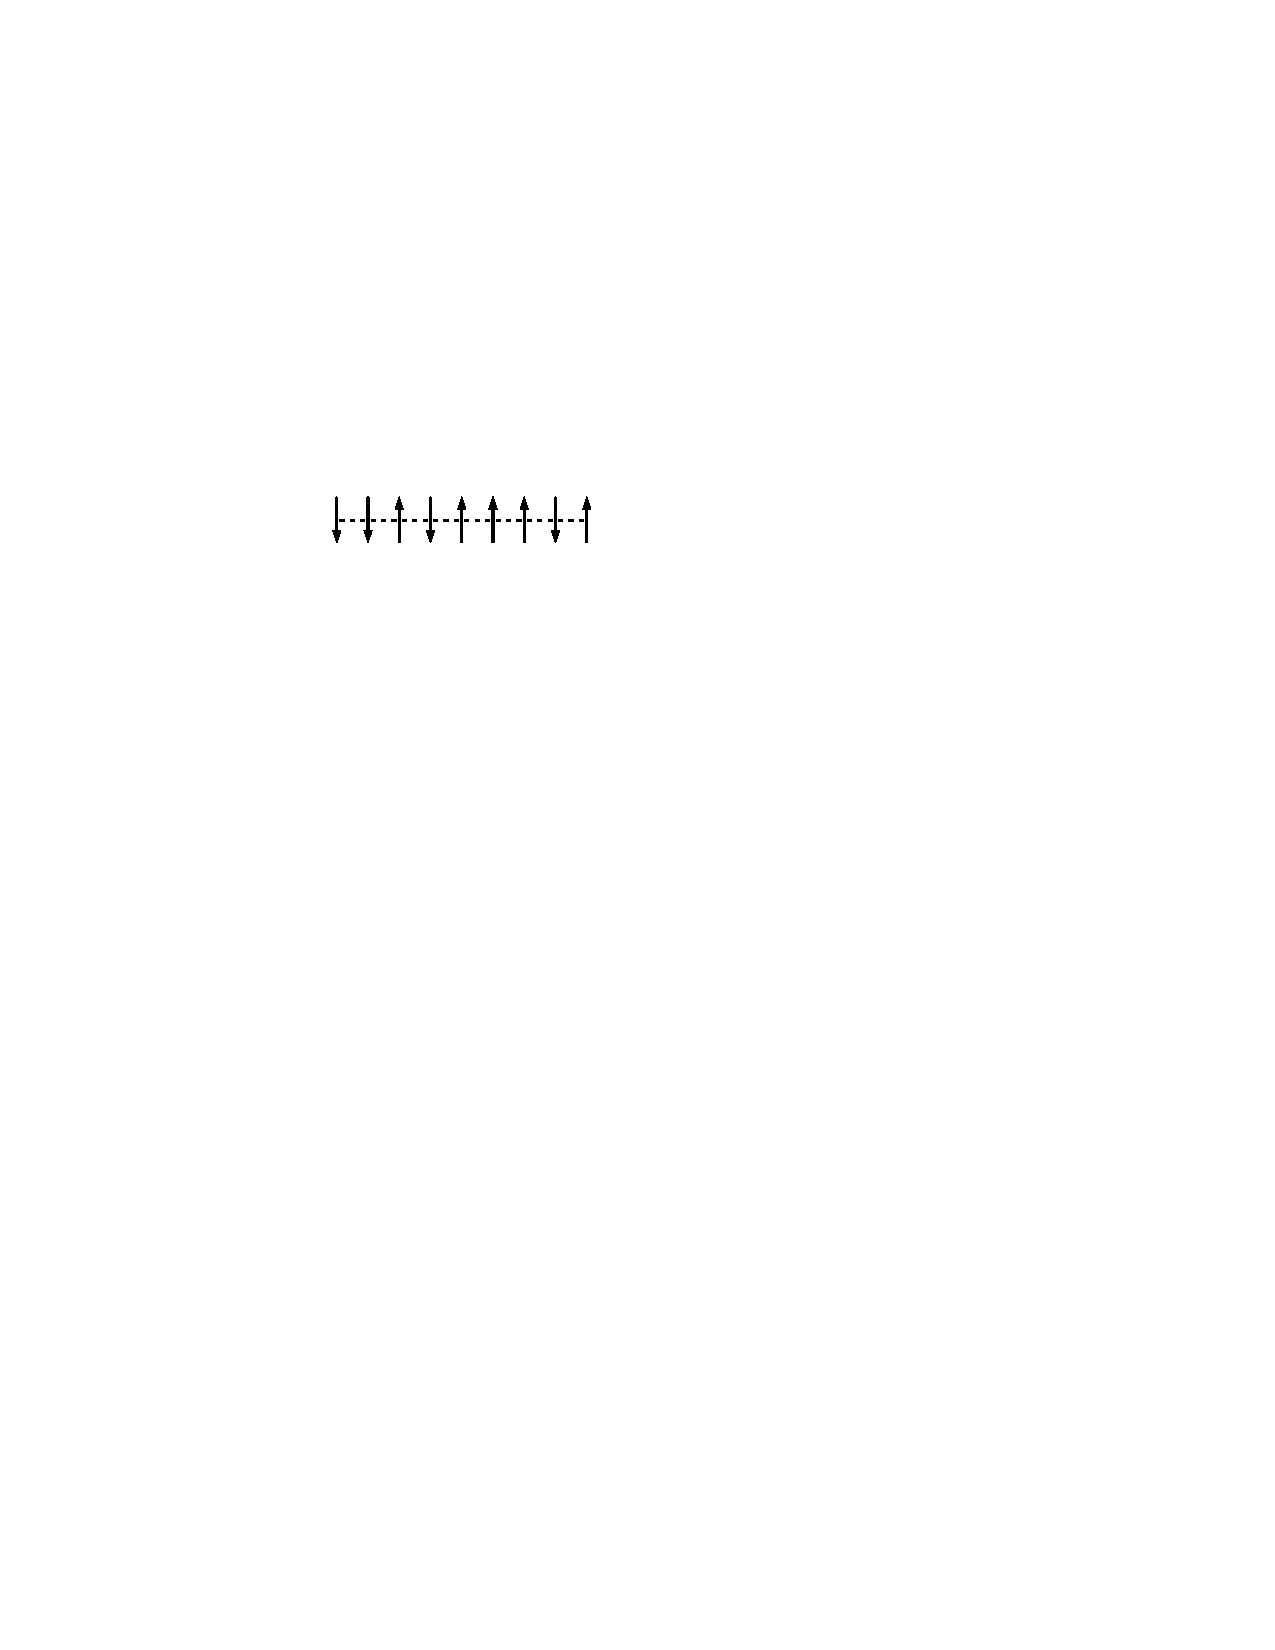
\includegraphics[width=\textwidth]{../Lecture5/Ising-spins-1D.pdf}
  \end{figure}

\end{frame}

%-----------------------------------------------------------------------------------------

\begin{frame}%[shrink=10]
  \frametitle{Ising's analytic solution for a 1D spin lattice (II)}

    We can generalize this to $N$ spins, either by induction based on one more manual sum with $N=3$, or by direct proof (which I leave to you!)
%
  \begin{eqnarray}
    Z_3 &=& \sum_{s_1 = \pm1} \sum_{s_2 = \pm1} \sum_{s_3 = \pm1} e^{ \beta J\sum_{i=1}^{N-1} s_i s_{i+1} } \\ \pause
        &=& \sum_{s_1 = \pm1} \sum_{s_2 = \pm1} \sum_{s_3 = \pm1} e^{ \beta J s_1 s_2 + \beta J s_2 s_3 } \\ \pause
        &=& \sum_{s_1 = \pm1} \sum_{s_2 = \pm1} e^{ \beta J s_1 s_2} \left[ e^{ \beta J s_2 } + e^{- \beta J s_2 } \right] \\ \pause
        &=& 2 \cosh \beta J \sum_{s_1 = \pm1} \sum_{s_2 = \pm1} e^{ \beta J s_1 s_2}  \\ \pause
        &=& \left(2 \cosh \beta J\right) Z_2 \\ \pause
    Z_N &=& \left(2 \cosh \beta J\right) Z_{N-1} \\ \pause
        &=& \left(2 \cosh \beta J\right)^{N}
  \end{eqnarray}
  %
  (Since $Z_1 = \sum_{s_1 = \pm1} 1 = 2$)
  
\end{frame}

%-----------------------------------------------------------------------------------------

\begin{frame}%[shrink=10]
  \frametitle{Results using Ising's analytic model (I)}

    With the expression for $Z$, we can calculate key properties of the system
%
  \begin{eqnarray}
    \mean{E} &=& -\frac{1}{Z}\frac{\partial Z}{\partial\beta} = -\frac{\partial \ln Z}{\partial\beta} \\ \pause
             &=& -\frac{1}{\left(2 \cosh \beta J\right)^{N}}\frac{\partial \left[\left(2 \cosh \beta J\right)^{N}\right]}{\partial\beta} \\ \pause
             &=& -N\frac{\left(2 \cosh \beta J\right)^{N-1}}{\left(2 \cosh \beta J\right)^{N}}\left(2J \sinh \beta J\right) \\ \pause
             &=& -NJ\tanh \beta J 
  \end{eqnarray}
  %
  
\end{frame}

%-----------------------------------------------------------------------------------------

\begin{frame}%[shrink=10]
  \frametitle{Results using Ising's analytic model (II)}

    Without completing a more thorough derivation, here are three more key properties of the system:
    \begin{itemize}
      \item<1-> \bluebf{$F$:  Helmholtz free energy}, measures the useful work obtainable from a closed thermodynamic system at a constant $T$ and volume. Analogous to Gibbs free energy, which does the same at constant pressure.
      \item<2-> \bluebf{$C$: Heat capacity}, measures the system's response to changes in $T$
      \item<4-> \bluebf{$M$: Magnetization}, measures the amount of aligned spins in the system
    \end{itemize}
%
  \begin{eqnarray}
           F &=& -\frac{1}{\beta} \ln Z = -\frac{N}{\beta} \ln (2 \cosh \beta J) \\ \pause   
           C &=& \frac{\partial \mean{E}}{\partial T} = -\kB \beta^2 \frac{\partial^2 \ln Z}{\partial \beta^2} = \frac{N (\beta J)^2}{\cosh^2 \beta J} \pause \textcolor{red}{\left(= \kB \beta^2 Var(E) \right)} \label{eq:specificheat} \\  \pause 
           M &=& -\frac{\partial F}{\partial H} = \frac{N \sinh \beta H}{\sqrt{\sinh^2 \beta H + e^{-4 \beta J}}}  \pause \textcolor{red}{\left(= \sum_i \spini \right)}  \label{eq:magnetization}
  \end{eqnarray} 
  %
  \pause
  %
  \textit{Note: at constant $T$, Helmholtz free energy ($F$) is minimized at equilibrium.}
  
\end{frame}

%-----------------------------------------------------------------------------------------

\begin{frame}%[shrink=10]
  \frametitle{(lack of) Phase transition for 1D model}

  The last expression for magnetization $M$, or magnetization per unit particle, $m=M/N$ shows a very important property
  %
  \begin{eqnarray}
           M &=& -\frac{\partial F}{\partial H} = \frac{N \sinh \beta H}{\sqrt{\sinh^2 \beta H + e^{-4 \beta J}}} 
  \end{eqnarray}
  %
  \begin{itemize}
    \item $M=0$ for $H=0$ because $\sinh x \approx x$ for small $x$
    \item For $H=0$, $\sinh \beta H = 0$ and thus $M = 0$
    \item 1D Ising model becomes a ferromagnet only at $T =0$ where $e^{-4 \beta J} \ra 0$, and thus $|M| \ra 1$ at $T =0$.
  \end{itemize}
  
  \pause
  
  \begin{ucblock}{}
  \centering \bluebf{There is no state above $T=0$ for which the mean magnetization is non-zero, while at $T=0$, we see that $M\ra 1$ and the system exhibits a \alertbf{phase transition} (we will come back to this).} 
  \end{ucblock}
  %
  \pause
  %
  \begin{figure}
    \center 
    \frame{\includegraphics[width=\textwidth]{NonFerromagneticStatement.pdf}}
    \href{https://journals.aps.org/pr/abstract/10.1103/PhysRev.60.252}{Kramers \& Wannier, 1941}
  \end{figure}
  
\end{frame}

%-----------------------------------------------------------------------------------------
\subsection[2D Ising Model]{2D Ising Model}
%-----------------------------------------------------------------------------------------

%-----------------------------------------------------------------------------------------

\begin{frame}%[shrink=10]
  \frametitle{Properties of the 2D Ising model}
  \framesubtitle{\href{https://journals.aps.org/pr/abstract/10.1103/PhysRev.65.117}{Lars Onsager, Phys. Rev. 65, 117 -- Published 1 February 1944}}

  Onsager showed in 1943 that one can solve the 2D Ising model analytically.
  
  %\vspace{-0.4cm}
  
  \begin{columns}
  
    \column{0.55\textwidth}
    
      Solution for $\ln {Z/2} = -\beta F - \ln 2$ (and allowing different $J$ in each dimension)
      
      \begin{figure}
        \frame{\includegraphics[width=0.9\columnwidth]{OnsagersSolutionFreeEnergy.pdf}}
      \end{figure}
      
      This leads to a relationship for the magnetization which \alert{does allow for $M\neq0$ at $T\neq0$, namely $T=T_c$}:
      
      \begin{equation}
        \sinh \left( \frac{2 J_1}{\kB T_c} \right) \sinh \left( \frac{2 J_2}{\kB T_c} \right) = 1
      \end{equation}
      
      
      
    \column{0.45\textwidth}
    
      \begin{figure}
        \centering
        \includegraphics[width=\columnwidth]{OnsagersIsingModel2.pdf}
      \end{figure}
    
      \pause
    
      Which corresponds to
      
      \begin{eqnarray}
         \frac{\kB T_{c}}{J} &=& {\frac {2}{\ln(1+{\sqrt {2}})}} \\
                             &=& 2.2692
      \end{eqnarray}
  
  \end{columns}  
  
\end{frame}

%==========================================================================================
\section[Ising model observables and calculations]{Ising model observables and calculations}
%==========================================================================================

%-----------------------------------------------------------------------------------------
\subsection[Equilibrium]{Equilibrium}
%-----------------------------------------------------------------------------------------

\begin{frame}%[shrink=10]
  \frametitle{Equilibration time}
  
  Before we can \alertbf{``reliably''} measure something about a simulated system, we have to wait for the system to reach a sort of ``steady state''...why is that?
  
  \pause
  
  \vspace{0.3cm}
  
  \begin{ucblock}{}
    \centering \LARGE Equilibrium
  \end{ucblock}
  
  \vspace{0.3cm}
  
  \pause
  
  In order to measure properties of the system using a simulation, we have to run our simulation for a suitably long period of time until it has come to equilibrium at the temperature (or whatever state-related property) we are interested in. This period is called the equilibration time $\tau_{\mathrm{eq}}$. 
  
  \vspace{0.3cm}
  
  Only then can we obtain a reliable measurement of the quantity we are interested in. And then, in order to measure it's average values we must wait another suitably long period of time and average it, to evaluate the estimator of that quantity. 
  
\end{frame}

%-----------------------------------------------------------------------------------------

\begin{frame}%[shrink=10]
  \frametitle{So many questions!}
  
  \begin{ucblock}{Questions you should ask yourself}
    \begin{itemize}
      \item What exactly do we mean by ``allowing the system to come to equilibrium''? 
      \item How long is a ``suitably long time'' for it to happen? 
      \item How do we go about measuring our quantity of interest once that happens?
      \item How long do we have to average over to get a result of a desired degree of accuracy?
    \end{itemize}
  \end{ucblock}
  
  \vspace{0.3cm}
  
  \centering \bluebf{These are very general questions which we need to consider every time we do a Monte Carlo simulation. }

\end{frame}

%-----------------------------------------------------------------------------------------

\begin{frame}%[shrink=10]
  \frametitle{Discussion of equilibrium}
 
  \bluebf{``Equilibrium'}' means that the average probability of finding our system in any particular state $\mu$ is proportional to the Boltzmann weight $e^{-\beta E_{\mu}}$ of that state.
  
  \vspace{0.3cm}

  If we start our system off in a state such as with $T = 0$ (e.g. all spins aligned), and we want to perform a simulation at some finite non-zero temperature, $T\neq0$, it will take a little time before we reach equilibrium.
  
  \vspace{0.3cm}

A system at equilibrium spends the overwhelming majority of its time in a small subset of states in which its internal energy and other properties take a narrow range of values. This is what is ``mapped out'' by the temperature. To determine if the system has reached equilibrium, we could just ``look at it'' but this isn't very reliable. 

\end{frame}

%-----------------------------------------------------------------------------------------
\subsection[Magnetization]{Magnetization}
%-----------------------------------------------------------------------------------------

\begin{frame}%[shrink=10]
  \frametitle{Equilibrium in simulations: magnetization}
 
  A standard approach is to plot a graph of some quantity of interest, like the magnetization per spin $m=M/N$ of the system or the energy of the system $E$, as a function of ``time'' (iterations or steps) from the start of the simulation. 
  
  \vspace{0.3cm}
  
  Up until equilibrium, the energy and the magnetization are changing, but after equilibrium is reached, they just fluctuate around a steady average value. This is what we should measure.
  
  \begin{figure}
    \includegraphics[width=0.6\columnwidth]{MagnetizationVsTime.pdf}
  \end{figure}
 
\end{frame}


%-----------------------------------------------------------------------------------------

\begin{frame}%[shrink=10]
  \frametitle{Simulation vs. calculations for the 2D Ising model}

  \begin{figure}
    \includegraphics[width=0.47\columnwidth]{2DIsing-Simulation-MagnetizationSpecificHeat.pdf}
    \includegraphics[width=0.47\columnwidth]{2DIsing-Simulation-Magnetization.pdf}
  \end{figure}
  %
  \vspace{-0.5cm}
  %
  These results come from \alertbf{two simulations (markers)}, a $5\times 5$ lattice (left) and a $100\times 100$ lattice (right). These are compared to \bluebf{analytic calculations (solid lines)}. Many iterations are run for each simulation, and averaged after equilibrium is reached to measure the magnetization and the energy. $m=M/N$ and $c=C/N$ are obtained from Eqs~\ref{eq:specificheat},\ref{eq:magnetization}, and $J=\kB=1$. 
  %
  %\vspace{-0.5cm}
  %
  \begin{ucblock}{}
    \centering The features at the Curie temperature $T_c$ are an indication of a \alertbf{phase transition}, for which the magnetization is the \alertbf{order parameter}
  \end{ucblock}
  
\end{frame}


%-----------------------------------------------------------------------------------------
\subsection[Specific heat]{Specific heat}
%-----------------------------------------------------------------------------------------

%-----------------------------------------------------------------------------------------

\begin{frame}%[shrink=10]
  \frametitle{Specific heat: a measure of the variance of the energy}
 
  As we wrote down in Eq.~\ref{eq:specificheat}:
  
  \begin{equation}
    C = \frac{\partial \mean{E}}{\partial T} = -\kB \beta^2 \frac{\partial^2 \ln Z}{\partial \beta^2} = \frac{N (\beta J)^2}{\cosh^2 \beta J}  \textcolor{red}{\, = \kB \beta^2 Var(E) }   
  \end{equation}
  %
  we can calculate this in terms of the energies of the system.
  %    
  \begin{figure}
    \includegraphics[width=0.6\columnwidth]{2DIsing-Simulation-SpecificHeat.pdf}
  \end{figure}
  %
  \vspace{-0.2cm}
  \begin{ucblock}{}
    \centering The divergence at $T_c$ is another indication of a \alertbf{phase transition}
  \end{ucblock}
  
\end{frame}

%-----------------------------------------------------------------------------------------
\subsection[Phase transition]{Phase transition}
%-----------------------------------------------------------------------------------------

%-----------------------------------------------------------------------------------------

\begin{frame}%[shrink=10]
  \frametitle{Phase transitions}
 
  \begin{columns}
  
  \column{0.55\textwidth}
 
  We have all heard of, talked about, played with, and even tasted phase transitions since shortly after we were born:
  
  \vspace{0.5cm}
  
  \begin{ucblock}{Basic idea of a phase transition (Wikipedia)}
    A phase of a thermodynamic system and the states of matter have uniform physical properties. During a phase transition of a given medium, certain properties of the medium change, often discontinuously, as a result of the change of some external condition, such as temperature, pressure, or others. 
  \end{ucblock}
  %
  \column{0.45\textwidth}
  
  \begin{figure}
    \includegraphics<1>[width=\columnwidth]{PhasesWater.png}
    \includegraphics<2>[width=\columnwidth]{Phase-diag2.png}
  \end{figure}
  %
  %
  \end{columns}
  
\end{frame}

%-----------------------------------------------------------------------------------------

\begin{frame}%[shrink=10]
  \frametitle{More exotic phase transitions}

  \begin{columns}
  
  \column{0.55\textwidth}
 
  What you have likely \alertbf{not heard of or talked about}, certainly have not \alertbf{``played with''}, and \alertbf{definitely have not tasted} \bluebf{phase transitions in the early universe (or at the LHC)}:
  
  \vspace{0.5cm}
  
  \column{0.45\textwidth}
  
  \begin{figure}
    \includegraphics[width=\columnwidth]{LHCPhaseTransition.jpg}
  \end{figure}
  %
  %
  \end{columns}

  \vspace{0.3cm}

  In each case, the description of the system has gross characteristics that depend on certain parameters, and very often, some notion of \alertbf{temperature}.
  
\end{frame}

%-----------------------------------------------------------------------------------------

\begin{frame}%[shrink=10]
  \frametitle{Let's look at that plot of magnetization again}

  \begin{columns}
  
  \column{0.35\textwidth}
 
  Pretty clear that there is a phase transition occuring!
  
  \vspace{0.5cm}
  
  \column{0.65\textwidth}
  
  \begin{figure}
    \includegraphics[width=\columnwidth]{2DIsing-Simulation-Magnetization.pdf}
  \end{figure}
  %
  %
  \end{columns}

  
\end{frame}

%==========================================================================================
\section[Hints for HW3]{Hints for HW3}
%==========================================================================================

\begin{frame}[fragile,shrink=15]
  \frametitle{Some hints for HW3}

  We'll work on this together tomorrow (remember, CSIL at 2:30pm!) but here are some hints in the mean time
  
  \vspace{0.3cm}
  
  \begin{ucblock}{Approach}
    Make sure you have short snippets that allow you to test each function you write and make sure it's doing what you think it should be doing. 
  \end{ucblock}
  
  \begin{ucpythonblock}{Spin sums}
     # Can be used instead of my example code for 
     # less readable, but much faster sums
     np.roll(lattice) 
  \end{ucpythonblock}
  
  \begin{ucpythonblock}{Energy variance}
     # Useful for specific heat 
     # Modularize your manipulations of the lattice!
     np.var(energy_density/(T**2))
  \end{ucpythonblock}
  
  \begin{ucblock}{Equilibrium}
    Test the ``time'' required to reach equilibrium \alertbf{before} doing many simulations with many iterations each.
  \end{ucblock}
  
\end{frame}



%
%For a $30\times30$ lattice with 20,000 time steps per simulation, I was seeing 2.5s/simulation or about 2-3 min to run 100 simulations at different temperatures

%%==========================================================================================
%\section[Conclusions]{Conclusions}
%==========================================================================================
%
%\begin{frame}%[shrink=1]
%  \frametitle{Conclusions}
%
%  \begin{itemize}
%    \item Something
%  \end{itemize}
%  
%\end{frame}

%==========================================================================================
%==========================================================================================
\end{document}
